% $Id: $
\documentclass[a4paper,11pt]{article}
\usepackage{a4wide}

\usepackage{amsmath,amsthm}
\usepackage{amsfonts}
% The following makes latex use nicer postscript fonts.
\usepackage{times}
\usepackage{subcaption}
\usepackage[english]{babel}
%\usepackage[colorlinks,urlcolor=blue,linkcolor=blue]{hyperref}
\pagestyle{headings}
\usepackage{vubtitlepage}
\usepackage{lmodern}

\usepackage[geometry]{ifsym}
%\usepackage[font=small,format=plain,labelfont=bf,up,textfont=it,up]{caption}
\renewcommand{\thefigure}{\thesection.\arabic{figure}}

\author{Filip Moons}
\title{Game Theory: Distributed Selfish Load Balancing on Networks}
\newtheorem{theorem}{Theorem}[section]
\newtheorem{lemma}[theorem]{Lemma}
\newtheorem{proposition}[theorem]{Proposition}
\newtheorem{conjecture}{Conjecture}
\newtheorem{example}[theorem]{Example}
\newtheorem{property}[theorem]{Property}
\newtheorem{definition}[theorem]{Definition}
\newtheorem{corollary}[theorem]{Corollary}
\newtheorem{remark}[theorem]{Remark}
\newtheorem{examples}[theorem]{Examples}
\newtheorem{remarks}[theorem]{Remarks}
\newtheorem{notation}[theorem]{Notation}
\setcounter{tocdepth}{5}   
\newcommand{\N}{{\mathbb N}}
\newcommand{\Z}{{\mathbb Z}}
\newcommand{\Q}{{\mathbb Q}}
\newcommand{\R}{{\mathbb R}}
\newcommand{\C}{{\mathbb C}}
\newcommand{\HQ}{{\mathbb H}}
\renewcommand{\P}{{\mathbb P}}
\newcommand{\E}{{\mathbb E}}
\newcommand{\cost}{\text{cost}}
\newcommand{\Nash}{\text{Nash}}
\newcommand{\nash}{\text{nash}}
\newcommand{\opt}{\text{opt}}
\newcommand{\copt}{\cost(a_{\opt})}
%\newenvironment{proof}{\noindent{\bf Bewijs.}}{{\hfill $ \Box $}\vskip 4mm}

%\promotortitle{Promotor/Promotors}
\promotor{Prof. Dr. Ann Now\'{e}}
\advisors{}
\advisortitle{}
\addto\captionsenglish{\renewcommand*\abstractname{Abstract for non-mathematicians}}
\date{MEI 2006}
\faculty{Faculty of Science}
\advisortitle{}
\department{Department of Mathematics}
\reason{Bachelor Thesis I}

\date{January 2013}


\begin{document}
% Then english TitlePage
\maketitlepage
\newpage
\null\vspace{\fill}

\begin{abstract}
Explaining the subject of my Bachelor thesis to those who do not study either Mathematics or Computer Science isn't an easy task, but I can give an idea of the problem studied by giving an example. Imagine, for example, that there are only two roads from Paris to Brussels: road A \& road B. If you take road A you'll always drive 5 hours, independent from the usage of road A by other drivers (\emph{agents} is the more game theoretical word). If you take road B, the time you need depends of the number of other agents using road B: you'll drive $5\frac{x}{100}$ hours, with $x$ the number of agents, but also on this road the maximum time spend is 5 hours, so mathematically that becomes $\min(5, 5\frac{x}{100})$ hours. Because every agent acts selfish and rational, the result under this circumstances and with only this information will be that every agent will take at any time road B: with road A they drive always 5 hours, with road B there is a chance to get to Brussels in less time. But consider now the following situation: exact 100 agents decide at the same time to go to Brussels, that means that all of them will take road B and so everyone will drive 5 hours. It would be much better that 50 agents would take road A (and thus drive 5 hours) and the other 50 take road B (and drive $5\frac{50}{100} = 2.5$ hours), that would reduce the average time to $3.75$ hours! This kind of problems where the selfishness of agents reduce the power (load) of a general system take place in a wide range of real life problems: not only in traffic, but also in economics, politics and, that's more my interest, also in Computer Science: in a distributed system computers interact on a selfish base because there isn't a central computer that organizes the network. It's extremely interesting to study which information these kind of agents (computers) need to know to reduce their selfishness and reach the optimal power of the distributed network.
\end{abstract}
\vspace{\fill}
\newpage

\tableofcontents
\newpage


\section{Introduction}
Whenever a set of task should be executed on a set of resources, the problem of load balancing evidently arouses. We need to balance the load among the resources in order to exploit the available resources efficiently and fair.
\subsection{Why we need Game Theory}
 One of the most fundamental load balancing problems is \emph{makespan scheduling on uniformly related machines}. This problem is defined by $m$ machines with speeds $s_1,...s_m$ and $n$ tasks with weights $w_1,...,w_n$. Let $[n] = \{1,...,n\}$ be to set of tasks and $[m]$ the set of machines. Now, the problem is to find an assignment function $A: [n] \rightarrow [m]$ of the tasks to the machines that is as balanced as possible. The load of machine $j \in [m]$ under $A$ is defined as:
\begin{displaymath}
  \ell_j = \displaystyle\sum_{\substack{i \in [n] \\j = A(i)}}{\frac{w_i}{s_j}}
\end{displaymath}

The \emph{makespan} is defined as $$\max\limits_{j \in [m]}(\ell_j)$$

Now, of course, the objective is to minimize the makespan. When there is a central machine, it ins't that hard to design algorithms that compute a mapping A that minimizes the makespan. Suppose, however, that there is not a central machine that can enforce an efficient mapping of the tasks to the machines (e.g. in P2P Networks). This naturally leads to the following game theoretic setting in which we will be able to analyze what happens to the makespan if there is no global authority but selfish agents aiming at maximizing their individual benefit decide about the assignment of tasks. The understand the problem and it's solution, we first give the most important game theoretical results you'll need.

\section{Introducing Load Balancing Games}
Important note: This section doesn't aim to give the reader an introduction in Game Theory. Instead, it gives only the relevant results that the reader must know for understanding the rest of this paper.

\subsection{Strategic games}
\subsubsection{Defenition}
\begin{definition}\cite{2}
A strategic game $\langle N, (A_i), \succeq_i\rangle$ consists of:
\begin{itemize}
  \item a finite set $N$  (the set of \textbf{players}),
  \item for each player $i \in N$ a nonempty set $A_i$ (the \textbf{set of actions} available to player i),
  \item for each player $i \in N$ a preference relation $\succeq_i$ on $A=\times_{j\in N}A_j$ (the \textbf{preference relation} of player i).
\end{itemize}
\end{definition}
\begin{remark}
Under a wide range of circumstances the preference relation  $\succeq_i$ of player $i$ in a strategic game can be represented by a \textbf{payoff function} $u_i: A \rightarrow \R$, in the sense that $u_i(a) \geq u_i(b)$ whenever $a \succeq_i b$. Sometimes this function is also called a utility function. A strategic game is then often denoted as $G = \langle N, (A_i), (u_i)\rangle$. In this paper, we assume that every strategic game has a payoff function, because the more general case is irrelevant for the subject studied.
\end{remark}


\subsubsection{Mixed and pure strategies}
A \emph{pure strategy} provides a complete definition of how a player will play a game. In particular, it determines the action a player will make for any situation he or she could face. Mathematically, an element $a = (a_1,...,a_n) \in A$ is called \emph{pure strategy profile}. The components $a_i$ of $a$ contain an action for each player at any stage of the game.

A \emph{mixed strategy} is an assignment of a probability to each action that is available to the player. This allows for a player to randomly select a pure strategy. Since probabilities are continuous, there are infinitely many mixed strategies available to a player, even if their strategy set is finite.

Of course, one can regard a pure strategy as a degenerate case of a mixed strategy, in which that particular pure strategy is selected with probability 1 and every other strategy with probability 0.

Let in a \emph{mixed strategy}, $\alpha_i(a_j)$ (with $a_j \in A_i$) denote the probability that player $i$ choose action $j$, thus: $\alpha_i(a_j) = \P[A_i = a_j]$. A \emph{mixed strategy profile} $$\alpha = \left(\alpha_i\right)_{i\in N}$$ specifies the probabilities for all players for all their possible actions. The probability of obtaining a specific pure strategy profile $a = (a_1,...,a_n)$ is:
$$\P[\alpha = A] = \displaystyle\prod_{i \in N} \alpha_i(a_i)$$
 We can now define the \emph{expected payoff} for player $i$ under a mixed strategy profile $\alpha$:
$$U_i(\alpha) = \displaystyle\sum_{a \in A}{\left(\prod_{j \in N}{\alpha_j(a_j)}\right) u_i(a)}$$
Or, by using the properties of the (discrete) expected value (we iterate over the pure strategy profiles $a \in A$)\footnote[1]{This notation is a little bit ambiguous, because in advanced game theory, also the payoff function may have a distribution. The reader must keep in mind that in this paper, payoff functions do not have a distribution.}:
$$U_i(\alpha) = \E[u_i(a)]$$ 
The set of all mixed strategy profiles in a strategic game for a specific player $i$ is denoted as $\Delta(A_i)$. Note that $(\alpha_i(a_1),...,\alpha_i(a_k),...)$ with the $a_j$'s the pure actions of player $i$ (thus $a_j \in A_i$) are the (vector)elements in $\Delta(A_i)$. The set of all mixed strategy profiles in a strategic game is denoted as $\Delta(A)$ and is defined as: $\Delta(A) = \Delta(A_1) \times ... \times \Delta(A_n)$ .


\subsubsection{Nash Equilibra}
One of the most fundamental concepts in game theory is that of Nash equilibrum. This notion captures a steady state of the play of a strategic game in which no player can improve his cost by unilaterally changing his strategy. Of course, we distinguish pure and mixed Nash Equilibra.

\begin{definition}(Pure Nash Equilibrum) \cite{6}
A pure strategy profile $a^* \in A$ is a \textbf{pure Nash Equilibrum} if for each player $i\in N$:
$$u_i(a_{-i}^*,a_i^*)) \geq u_i(a_{-i}^*, a_i) \;\;\;\; \forall a_i \in A_i$$
\end{definition}

\begin{definition}(Mixed Nash Equilibrum)\cite{10}
A mixed strategy profile $\alpha^*$ is a \textbf{mixed Nash Equilibrum} if for each player $i \in N$:
$$U_i(\alpha_{-i}^*,\alpha_i^*)) \geq U_i(\alpha_{-i}^*, \alpha_i) \;\;\;\; \forall \alpha_i$$
\end{definition}

\begin{remark}\label{herordening}
The notation $(a_{-i}^*, a_{i})$ for a pure strategy profile $a^*$ is a slight abuse of notation that is quite common in Game Theory, meaning that $a_i^* \in A_i$ and $Sa_{-i} \in A_1\times ... \times A_{i-1} \times A_{i+1} ... \times A_n$. The same holds for the mixed strategy profiles. It's important to realize that players have no exact order in a strategy profile, so they can always be re-ordered.
\end{remark}

Although there is not enough space to give a deep explanation of the concept of a Nash equilibrum, it's important to know that a Nash equilibrum is not necessary an optimal solution of a game. It's only a profile in which no player will benefit from changing his strategy on it's own.

\subsubsection{Theorem of Nash}
Now we have defined the concept of Nash Equilibrum, we can look at one of the most fundamental theorems in Game Theory: \emph{the Theorem of Nash}. This theorem states that every finite strategic game has at least one mixed Nash Equilibrum.

Nash proofed his theorem in 1950 by using the Brouwer fixed point theorem. Later on, a lot easier version of the proof is found by using the Kakutani's fixed point theorem. However, the (one dimensional version of) the Brouwer fixed point theorem is much more familiar because it's proved in almost every intermediate Analysis course. Therefore, we will give the original proof of Nash.

\begin{definition}(Fixed point)\cite{11}
Let $X$ be a set and $f: X \rightarrow X$ a function. A point $x \in X$ is called a \textbf{fixed point} of $f$ if $f(x)=x$.
\end{definition}

\begin{property}(One dimensional version Brouwer fixed point theorem) \cite{11}
 Every continuous function $$f: [a,b] \rightarrow [a,b]$$  has a fixed point.
\end{property}
\begin{proof}
As the codomain of $f$ is $[a,b]$ it follows that the image of $f$ is a subset of $[a,b]$. Thus $f(a) \geq a$ and $f(b) \leq b$. Consider the function $$g: [a,b] \rightarrow \R: x \mapsto f(x) - x.$$
Then is $g$ also continuous and $g(a) \geq 0$ and $g(b) \leq 0$. By the theorem of Bolzano (see \cite{11}): $\exists c \in [a, b]: g(c) = 0$, but this means that $f(c) = c$.
\end{proof}
 The previous result is a very easy case of the Brouwer fixed point theorem. Proving the general theorem (see below) is very hard and falls behind the scope of this paper.
\begin{lemma}(Brouwer fixed point theorem)
Let $X$ be a non-empty, compact and convex set. If $f : X \rightarrow X$ is continuous, then there must exist $x \in X$ such that $f(x) = x$.
\end{lemma}

\begin{theorem}(Theorem of Nash)
Every finite strategic game has a mixed Nash equilibrum.
\end{theorem}

\begin{proof}
For every player $i$, let the set of actions $A_i$ is $\{a_{1}, ..., a_{m}\}$. For $1\leq i\leq n$. Let $\alpha$ be a mixed strategy profile of the the game and define $g_{ij}(\alpha)$ to be the gain for player $i$ form switching to his (pure) action $a_{j}$,:

$$g_{ij}(\alpha) = \max\{U_i(\alpha_{-i}, a_{j}) - U_i(\alpha),0\}$$

We can now define a map between mixed strategies of player $i$, $y:\Delta(A_i)\rightarrow \Delta(A_i)$ by

$$y_{ij}(\alpha) = \frac{\alpha_{i}(a_j)+g_{ij}(\alpha)}{1+\sum_{j=1}^{m}{g_{ij}(\alpha)}}$$

We now make two observations about this mapping:

\begin{itemize}
  \item For every player $i$ and his action $a_{j}$, the mapping $g_{ij}(\alpha)$ is continuous. This is due to the fact that $U_i(\alpha)$ is obviously continuous (it consist of the sum of products between a probability function and the continuous $u_i$), making $g_{ij}(\alpha)$ and consequently $y_{ij}(\alpha)$ continuous.

  \item For every player $i$, the vector $(y_{ij}(\alpha))_{j=1}^{m}$ is a distribution. This is due to the fact that the denominator of $y_{ij}(\alpha)$ is a normalization constant for any given $i$.


  \item Remember that $\Delta(A_i)$ has (vector)elements of the form $(\alpha_i(a_1),...,\alpha_i(a_k),...)$. Because the given strategic game is finite, we can identify $\Delta(A_i)$ with the set of vectors $(\alpha_i(a_1),...,\alpha_i(a_k))$, for which $\alpha_i(a_j) \geq 0 \;\; \forall j$ and $\sum^k_{j=1}{\alpha_i(a_j)} = 1$. We now proof that the set $\Delta(A_i)$ satisfies the conditions for the Brouwer fixed point theorem:
      \begin{itemize}
        \item The set $\Delta(A_i)$ is \emph{non-empty} by definition of a strategic game.
        \item To proof that the set $\Delta(A_i)$ is \emph{convex}, take $\vec{x} = (\alpha^x_i(a_1),...,\alpha^x_i(a_k))$ and $\vec{y} = (\alpha^y_i(a_1),...,\alpha^y_i(a_k))$ then $\vec{z} = \theta\vec{x} + (1 - \theta)\vec{y}$ for some $\theta \in [0,1]$ is in $\Delta(A_i)$ because $\vec{z}$ is also a mixed strategy for player $i$ (the sum of the components of $\vec{z}$ is 1).
        \item  The \emph{compactness} in $\R^k$ can be shown by proving that the set is closed and bounded. The set is bounded because $0 \leq \alpha_i(a_j) \leq 1$. To proof closeness in $\R^k$, we'll proof that the limit of every convergent sequence in $\Delta(A_i)$ is an element of $\Delta(A_i)$. Consider a convergent sequence in $\Delta(A_i): ((\alpha^n_i(a_1),...,\alpha^n_i(a_k))_n\rightarrow(\alpha^*_i(a_1),...,\alpha^*_i(a_k))$. Remember that a convergent sequence of vectors converges componentwise and that the addition is a continuous function, so:
            \begin{eqnarray*}
              \sum_{j=1}^k{\alpha^*_i(a_j)}  &=& \displaystyle\sum_{j=1}^k{\lim_{n\rightarrow\infty}{\alpha^n_i(a_j)}}\\
              &=& \displaystyle\lim_{n\rightarrow\infty}{\sum_{j=1}^k\alpha^n_i(a_j)}\\
              &=& \displaystyle\lim_{n\rightarrow\infty}{1}\\
              &=& 1
            \end{eqnarray*}
            this means that $(\alpha^*_i(a_1),...,\alpha^*_i(a_k))$ is also a mixed strategy for player $i$, but by definition of $\Delta(A_i)$, this limit belongs to $\Delta(A_i)$.
      \end{itemize}

\end{itemize}

Therefore $y$ fulfills the conditions of Brouwer's Fixed Point Theorem. Using the theorem, we conclude that there is a fixed point $\alpha*$ for $y$. This point satisfies

$$\alpha^*_{i}(a_j) = \frac{\alpha^*_{i}(a_j)+g_{ij}(\alpha^*)}{1+\sum_{j=1}^{m}{g_{ij}(\alpha^*)}}$$

Notice that this is possible only in one of two cases. Either $g_{ij}(\alpha)=0$ for every $i$ and $j$, in which case we have an equilibrium (since no one can profit from switching their strategy). If this is not the case, then there is a player $i$ such that $g_{ij}(\alpha)>0$. This would imply,

$$\alpha^*_{i}(a_j)\left(1+\sum_{j=1}^{m}{g_{ij}(\alpha^*)}\right) = \alpha^*_{i}(a_j)+g_{ij}(\alpha^*)$$

or

$$\alpha^*_{i}(a_j)\left(\sum_{j=1}^{m}{g_{ij}(\sigma)}\right) = g_{ij}(\alpha^*)$$.

This means that $g_{ij}(\alpha^*)=0$ if and only if $\alpha^*_{i}(a_j)=0$, and therefore, $\alpha^*_{i}(a_j)>0 \implies g_{ij}(\alpha*)>0$. However, this is impossible by the definition of $g_{ij}(\alpha)$. Recall that $U_i(\alpha)$ gives the expected payoff for a player under a mixed strategy $\alpha$. Therefore, it cannot be that player $i$ can profit from
`every' pure action in the support of $\alpha_i$ (with respect to $U_i(\alpha)$).

We are therefore left with the former possibility, i.e. $g_{ij}(\alpha)=0$ for all $i$ and $j$, implying a mixed Nash Equilibrium.
\end{proof}


\subsection{Congestion games}
\subsubsection{Definition}
Strategic games contains a wide range of games. We will now look at \emph{congestion games}: a specific kind of strategic games for which we can prove the existence of a pure Nash equilibrum. We will use this result for defining in the next section \emph{load balancing games}, a subclass of congestion games, this game is the one we'll need to handle the subject of this paper. Because we only need the theorem of the existence of a pure Nash equilibrum for congestion games, we will not take mixed strategies in consideration in this section.
\begin{definition}\cite{4,9}
A \textbf{congestion model} $(N, M, (A_i)_{i\in N}, (c_j)_{j\in M})$ is defined as follows:
\begin{itemize}
  \item a finite set $N$ of players. Each player $i$ has a weight (or demand) $w_i \in \N$,
  \item a finite set $M$ of facilities.
  \item For $i \in N$, $A_i$ denotes the set of strategies of player $i$, where each $a_i \in A_i$ is a non-empty subset of the facilities,
  \item For $j \in M, c_j$  is a cost function $\N \rightarrow \R$, $c_j(k)$ denotes the cost related to the use of facility $j$ under a certain load $k$;
\end{itemize}
\end{definition}
\begin{definition}\cite{2,4}
A \textbf{congestion game} associated with a congestion model is a strategic game with:
\begin{itemize}
  \item a finite set $N$ of players,
  \item for each player $i \in N$, there is a nonempty set of actions (strategies) $A_i$,
  \item the preference relation $\succeq_i$ for each player $i$ is defined by a payoff function $u_i: A \rightarrow \R$. For any $a \in A$ and for any $j \in M$, let $\ell_j(a)$ be \emph{the expected load on facility} $j$, assuming $a$ is the current pure strategy profile, so $\ell_j(a) = \sum_{\substack{i \in [n]\\j \in a_i}}{w_i}$ . Then the payoff function for player $i$ becomes: $u_i(a) = \sum_{j\in a_i} c_j(\ell_j(a))$.


\end{itemize}
\begin{remark}
Congestion models aren't always defined with the notion of weights of players (especially not in more economic game theory books). In those definitions, players have an equal weight. Those definitions match with ours if you give all players weight 1. Note that only the function $\ell_j(a)$ becomes much easier: it will just return the number of players using facility $j$ under a pure strategy profile $a$. From a computer scientific point of view, such definitions are not sufficient because players (\emph{tasks}) don't have the same weight. Watching the Eurovision Song Contest through a live stream is for example a much heavier task then sending an e-mail. 
\end{remark}
\begin{remark}\label{defcj}
In order to preserve the generality in the definition of congestion games, note that we only stated that $c_j$ are cost functions, without the need to explicitly define them. This is sufficient in this stage of the paper, however, the subject studied will require explicit definitions for $c_j$. These are given in section \ref{expdefcj}.
\end{remark}
\end{definition}
\subsubsection{The existence of a pure Nash equilbrum}
Rosenthal proved in 1973 that every congestion game has a pure Nash Equilibrum. The proof of this statement use the notion of a potential function. We will first define a potential function, give a concrete potential function for congestion games and proof that it holds the right properties. With this result we can then finally proof the existence of a pure Nash Equilibrum in congestion games.

\begin{definition}
Consider a function $\Phi: A \rightarrow \R$  defined on the space of pure stategy profiles of a (strategic) game $G$. If player $i$ switches unilaterally from $a_i$ to $a_i^*$, taking us from profile $a$ to profile $\vec{a^*}=(a_i^*, \vec{a_{-i}})$ and the following property holds:
$$\Phi(a) - \Phi(\vec{a^*}) = u_i(a) - u_i(\vec{a^*}) $$
then the function $\Phi$ is called a \textbf{potential function}.
\end{definition}



\begin{lemma}
The function
\begin{eqnarray*}
\Phi: A &\rightarrow& \R\\
a &\mapsto& \displaystyle\sum_{j=1}^{m}\displaystyle\sum_{k=1}^{\ell_j(a)} c_j(k)
\end{eqnarray*}
is a potential function for congestion games.
\end{lemma}

\begin{proof}(Rosenthal 1973)\cite{7,8}
In remark \ref{herordening} we already mentioned that players can be re-ordered. In particular, re-index player $i$ as player $n$ and vice versa.

Then, for $i' \in \{1,...,n\}$, define:
$$\ell_j^{i'}(a) = \displaystyle\sum_{\substack{l \in [1,...,i']\\j \in a_l}}{w_l} $$

Now, by using the commutativity, you can exchange the order of summation and become:
$$\Phi(a) = \displaystyle\sum_{i=1}^{n}\displaystyle\sum_{j\in a_i} c_j(\ell_j^i(a))$$

Denote that $\ell_j^n(a) = \ell_j(a)$, thus:
$$\displaystyle\sum_{j\in a_i} c_j(\ell_j^n(a)) = \displaystyle\sum_{j\in a_i} c_j(\ell_j(a)) = u_n(a)$$

So, if player $n$ switches from strategy $a_n$ to $a_n^*$, taking us from profile $a$ to profile $\vec{a^*}=(a_n^*, \vec{a_{-n}})$ then:

\begin{align*}
\Phi(a) - \Phi(\vec{a^*}) &= \!\left(\sum_{j\in a_1} c_j(\ell_j^1(a)) + ... + u_n(a) \!\right) - \!\left(\sum_{j\in a_1} c_j(\ell_j^1(\vec{a^*})) + ... + u_n(\vec{a^*}) \!\right)\\
\intertext{By definition of $\ell_j^i$, this becomes (the $n$'th player doesn't count for $\ell_j^i$ with $i < n$):}
&= \left(\sum_{j\in a_1} c_j(\ell_j^1(a)) + ... + u_n(a) \right) - \left(\sum_{j\in a_1} c_j(\ell_j^1(a)) + ... + u_n(\vec{a^*}) \right)\\
&= u_n(a) - u_n(\vec{a^*})
\end{align*}

We switched player $i$ with player $n$, so this holds for every player $i$.

\end{proof}

\begin{theorem}(Rosenthal 1973)\cite{7}\label{rosenthal}
Every congestion game has a pure Nash equilibrum.
\end{theorem}

\begin{proof}
Start from a random strategy vector $a$, and let repeatedly one player reduce it's costs. That means, that at each step $\Phi$ is reduced identically. Since $\Phi$ can accept a finite amount of values ($A$ is finite because it's the finite cartesian product of sets $A_i$ ($i \in \{1,...,n\}$), and every $A_i$ is finite because it's by definition a subset of the finite set of facilities $M$), this procedure will stop and reach a local minimum. At this point, no player can achieve any improvements, and we reach a pure \emph{Nash Equilibrum}.
\end{proof}



\subsection{Load balancing games}
\subsubsection{Definition}
Now we have introduced congestion games and proved that they always have a pure Nash Equilibrum, we take a closer look at a more specific kind of congestion games. Looking at the definition of a congestion game, it's immediately clear that this model is too general for giving a deeper understanding of the subject studied. Their is indeed a little problem with the actions (strategies) that a player can undertake: in a general congestion game, under a pure strategy profile $a$ the strategy of player $i$, $a_i$, consist of multiple facilities $j$. That means that the weight of a player (\emph{task}) counts for every function $c_j$ where $j \in a_i$. Of course, this is not realistic: a single task (\emph{player}) is not executed multiple times on different facilities. Therefore load balancing games are congestion games where the possible (pure) actions of players are singletons. So each $a_i = \{j\}$ ($i \in N, j \in M$) in a pure strategy profile $a \in A$. So, for every player $i$, $A_i \subset M$. In load balancing terminology, we use the terms \emph{machines} and \emph{tasks} instead of the terms facility and player.

\begin{definition}\cite{9}
A \textbf{load balancing game} is congestion game based on a congestion model with:
\begin{itemize}
  \item a finite set $N$ of tasks,
  \item for each player $i \in N$, there is a nonempty set of machines $A_i$ with $A_i \subset M$. The elements of $A_i$ are the possible machines on which task $i$ can be executed.
  \item the preference relation $\succeq_i$ for each client $i$ is defined by a payoff function $u_i: A \rightarrow \R$. For any $a \in A$ and for any $j \in M$, let $\ell_j(a)$ be \emph{the expected load on machine} $j$, assuming $a$ is the current pure strategy profile ($\ell_j(a) = \sum_{\substack{i \in [n]\\j = a_i}}{w_i}$) . Then the payoff function for task $i$ becomes: $u_i(a) = c_{a_i}(\ell_{a_i}(a))$.


\end{itemize}

\end{definition}
\section{Linear cost functions in Load Balancing Games}
Now we have defined \emph{load balancing games}, we can take a closer look at the subject studied. As already mentioned in remark \ref{defcj}, the cost functions in the previous section aren't explicitly defined. In this section we look at the situation where the cost functions $c_j$ for each machine $j$ are linear (thus of the form: $c_j(x) = \lambda_jx+\mu_j$ with $\lambda_j, \mu_j$ non-negative constants) and every server has a certain \emph{speed} $s_j \in N$.

\subsection{Payoffs and makespan}\label{expdefcj}
\subsubsection{Pure strategies}
In the most easy case, not only the players have a certain \emph{weight} $w_i \in N$, also the servers have certain \emph{speed} $s_j \in N$. Intuitively, such $s_j$ is the maximum amount of weight a server can handle. The cost functions $c_j$ can then easily be defined as:
$$c_j(k) = \frac{k}{s_j}$$

 The \textbf{\emph{payoff functions}} become then:
$$u_i(a) = c_{a_i}(\ell_{a_i}(a)) =  \frac{\ell_{a_i}(a)}{s_{a_i}}$$
The \emph{\textbf{social costs}} of a pure strategy is denoted as $\cost(a)$ and is defined to be the \emph{\textbf{makespan}}, i.e. $$\cost(a)=\max_{j\in[m]}{c_j(\ell_j(a))} = \max_{j\in[m]}{\frac{\ell_{j}(a)}{s_{j}}}$$


\subsubsection{Mixed strategies}
Of course, players may use mixed strategies. Let $x_i^j$ be a random variable for a mixed strategy profile $\alpha$ that takes the value $1$ if $a_i = j$. This means for pure strategy profiles:

\begin{eqnarray*}
\E[x^j_i(a)]    &=&  \displaystyle\sum_{a \in A}{\left(\prod_{j \in N}{\alpha_j(a_j)}\right) x^j_i(a)}\\
                &=& \displaystyle\sum_{a \in A}{\left(\prod_{j \in N}{\alpha_j(a_j)}\right) \delta_{a_i, j}}\\
                &=&  \displaystyle\sum_{a \in A}{\left(\P[\alpha = A]\right)\delta_{a_i,j}} \\
                &=& \P[A_i = j]\\
                &=& \alpha_i(j)\\
\end{eqnarray*}

Now we can also define $\ell_j$ on mixed strategies: $\ell_j: \Delta(A) \rightarrow \R$, we will define $\ell_j(\alpha)$ as the \textbf{expected load}:

\begin{eqnarray*}
\ell_j(\alpha)  &=& \E[\ell_j(a)] \\
                &=&  \displaystyle\sum_{a \in A}{\left(\prod_{k \in N}{\alpha_k(a_k)}\right) \ell_j(a)}\\
                &=& \displaystyle\sum_{a \in A}{\left(\prod_{k \in N}{\alpha_k(a_k)}\right) \sum_{\substack{i \in [n]\\j = a_i}}{w_i} }\\
                &=& \displaystyle\sum_{a \in A}{\left(\prod_{k \in N}{\alpha_k(a_k)}\right) \sum_{i \in [n]}{w_i\delta_{a_i,j}}}\\
                 &=&  \displaystyle\sum_{a \in A}{\left(\P[\alpha = A]\right)\sum_{i \in [n]}{w_i\delta_{a_i,j}}}\\
                &=& \sum_{i \in [n]}{w_i}\P[A_i = j]\\
                &=& \sum_{i \in [n]}{w_i}\alpha_i(j)
\end{eqnarray*}
$$\ell_j(\alpha) \E[\ell_j(\alpha)] = \E\left[\displaystyle\sum_{i \in [n]}{w_ix_i^j(\alpha)}\right] = \sum_{i \in [n]}{w_i\E[x_i^j(\alpha)]} = \sum_{i \in [n]}{w_i\alpha_i(j)}$$

The \emph\textbf{{social cost of a mixed strategy profile}} is defined as the \emph\textbf{{expected makespan}}:
$$\cost(\alpha) = \E[\cost(a)] = \E\left[\max_{j\in[m]}\frac{\ell_j(a)}{s_{j}}\right]$$

For mixed strategies, the expected payoff for player $i$, denoted by $U_i$ is defined as:
\begin{eqnarray*}
U_i(\alpha) &=& \E[u_i(a)]\\
  &=&  \displaystyle\sum_{a \in A}{\left(\prod_{k \in N}{\alpha_k(a_k)}\right) \frac{\ell_{a_i}(a)}{s_{a_i}}}\\
  &=&  \displaystyle\sum_{a \in A}{\left(\prod_{k \in N}{\alpha_k(a_k)}\right)\left(\sum_{j \in [m]}
 \frac{\ell_j(a)}{s_j}\delta_{a_i,j}\right)}\\
  &=&  \displaystyle\sum_{a \in A}{\left(\prod_{k \in N}{\alpha_k(a_k)}\right)\left(\sum_{j \in [m]}
  \frac{\sum_{\substack{l \in [n]\\j = a_l}}{w_i}}{s_j}\delta_{a_i,j}\right)}\\
  &=& \displaystyle\sum_{a \in A}{\left(\prod_{k \in N}{\alpha_k(a_k)}\right)\left(\sum_{j \in [m]}
\frac{\sum_{l \in [n]}{w_i\delta{a_l,j}}}{s_j}\delta_{a_i,j}\right)}\\
  &=&  \displaystyle\sum_{a \in A}{\left(\P[\alpha = A]\right)\left(\frac{\sum_{l \in [n]}{w_i\delta{a_l,1}}}{s_1}\delta_{a_i,1} + ... + \frac{\sum_{l \in [n]}{w_i\delta{a_l,m}}}{s_m}\delta_{a_i,m}\right)}\\
  &=&  \displaystyle\sum_{a \in A}{\left(\P[\alpha = A]\right)\left(\frac{\sum_{l \in [n]}{w_i\delta{a_l,1}}}{s_1}\delta_{a_i,1}\right)} + ... + \displaystyle\sum_{a \in A}{\left(\P[\alpha = A]\right)\left( \frac{\sum_{l \in [n]}{w_i\delta{a_l,m}}}{s_j}\delta_{a_i,m}\right)}\\
\end{eqnarray*}

From point of view of client $i$, the \emph{\textbf{expected cost on machine $j$}} under a mixed strategy profile $\alpha$, denoted by $U^j_i$, is:
\begin{eqnarray*}
U^j_i(\alpha) &=& \E[U_i(\alpha)|A_i=j]\\
  &=& \frac{w_i + \sum_{k\neq i}{w_k\alpha_k(j)}}{s_j} \\
  &=&  \frac{\ell_j(\alpha) + (1 - \alpha_i(j))w_i}{s_j}\\
\end{eqnarray*}
\subsection{An example of a Load Balancing Game with linear costs}
\begin{figure}
        \centering
        \begin{subfigure}{0.3\textwidth}
                \centering
                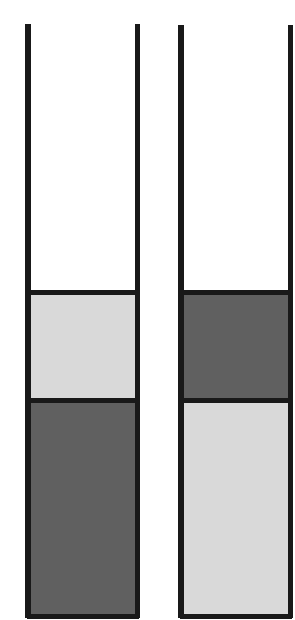
\includegraphics[scale=0.4]{figuura.pdf}
              \caption{Illustration of the optimal assignment}
                \label{fig:a}
        \end{subfigure}%
        ~ %add desired spacing between images, e. g. ~, \quad, \qquad etc. 
          %(or a blank line to force the subfigure onto a new line)
        \begin{subfigure}{0.3\textwidth}
                \centering
                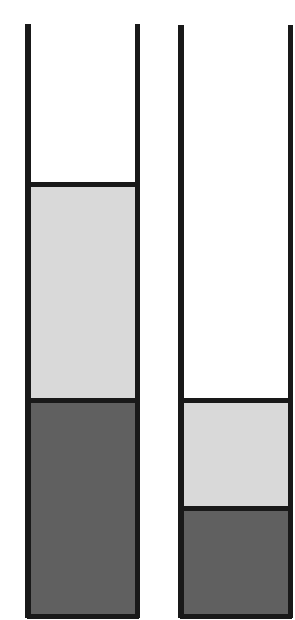
\includegraphics[scale=0.4]{figuurb.pdf}
                \caption{Illustration of a pure Nash equilibrum}
                \label{fig:b}
        \end{subfigure}
        \caption{(a) Illustration of the optimal assignment of an instance of the load balancing game with two large tasks of size 2 and two small tasks of size 1. The social cost of this assignment is 3. (b) Illustration of a pure Nash equilibrium for the same instance. The social cost of this assignment is 4, which is the maximum among all pure Nash equilibria for this instance.}
\end{figure}
After more than 10 pages theory, we give an easy example in which all introduced concepts are contained. 

Suppose that there are two identical machines both of which have speed $1$ and four tasks, two \emph{small tasks} of weight $1$ and two \emph{large tasks} of weight 2. An optimal assignment would map a small and a large task to each of the machines so that the load on both machines is $3$. This assignment is illustrated in figure \ref{fig:a}.

Now consider a pure strategy profile $a$ that maps the two large tasks to the first machines and the two small tasks to the second machine as illustrated in figure \ref{fig:b}. This way, the first machine has a load of $4$ and the second machine has a load of $2$. Obviously, a small task cannot improve its cost by moving from the second to the first machine. A large task cannot improve its cost by moving from the first tot the second machine either as its cost would remain 4 if it does. Thus this pure strategy profile $a$ constitutes a \emph{pure Nash equilibrium} with $\cost(a)=4$. This is beautiful example to show the already stated statement that Nash equilibra aren't mostly not the optimal situations. Observe that all assigments that yield a larger makespan than 4 cannot be a Nash equilibrium as, in this case, one of the machines has a load of at least $5$ and the other has a load of at most $1$ so that moving any task from the former to the latter would decrease the cost of this task. Thus, for this instance of the load balancing game, the social cost of the worst pure Nash Equilibrium is 4.

Clearly, the worst mixed equilibrium cannot be better than the worst pure equilibrium as the set of mixed equilibria is a superset of the set of pure equilibria, but can it really be worse? Suppose that each task is assigned to each of the machines with probability $\frac{1}{2}$. This corresponds to a mixed strategy profile $\alpha$ with the $\alpha_i$'s being constant functions, $$\alpha = \bigg(\underbrace{\frac{1}{2}}_{\alpha_1}, \underbrace{\frac{1}{2}}_{\alpha_2}, \underbrace{\frac{1}{2}}_{\alpha_3}, \underbrace{\frac{1}{2}}_{\alpha_4}\bigg) $$
. The expected load on machine $j$ is thus:
$$\ell_j(\alpha) = \displaystyle\sum_{1\leq i \leq 4}{w_i\alpha_i(j)} = \frac{1}{2} + \frac{1}{2} + 1 + 1 = 3$$
It's important to notice that te expected cost of a task on a machine is larger than the expected load of the machine, unless the task is assigned with probability 1 to this machine. For example, if we assume that task 1 is a small task, then:
$$U_1^j = \frac{\ell_j(\alpha) + (1 - \alpha_1(j))w_1} = 3 + \frac{1}{2} = 3.5$$
and, if task $3$ is a large task, then:
$$U_3^j = \frac{\ell_j(\alpha) + (1 - \alpha_3(j))w_3} = 3 + \frac{1}{2}.2 = 4$$
For symmetry reasons, the expected cost of each task under the considered mixed strategy profile $\alpha$ is the same on both machines so that $\alpha$ is a \emph{mixed Nash equilibrium}. The social cost of this equilibrium, $\cost(\alpha)$, is defined to be the expected makespan, $\E[cost(a)]$, of the random pure assignment $A$ induced by $\alpha$. The makespan, $\cost(a)$, is in fact a random variable. This variable can possibly take one of the four values $3, 4, 5$ or $6$. There are $2^4 = 16$ different assignments of four tasks to two machines. The number of assigments that yield a makespan of $3$ is $4$, 4 is 6, 5 is 4 and 6 is 2. Consequently, the social cost of the mixed Nash equilibrium is:
$$cost(\alpha) = \E[\cost(a)] = \frac{3.4 + 4.6 + 5.4+ 6.2}{16} = 4.25.$$
Thus mixed equilibria can, in fact, be worse than the worst pure equilibrium.

\subsection{The Price of Anarchy}
\subsubsection{Definition}
Since players (`tasks') act selfishly, load balancing games may reach assignments that do not minimize the makespan. We now introduce the notion of the \emph{\textbf{price of the anarchy}} to quantify the degradation of the overall system performance. 
\begin{definition}\cite{10}
Let \Nash(G) be the set of all (mixed) strategy profiles being a Nash equilibrium of a (load balancing) game $G$ and let $\alpha_{\opt}$ be the pure strategy profile being the social optimum. Then the \emph{\textbf{price of anarchy}} is defined as:
$$PoA(G) = \displaystyle\max_{\alpha \in \Nash(G)} {\frac{cost(\alpha)}{\cost(a_{\opt})}}$$
\end{definition}

The motivation behind studying the price of anarchy is to quantify the increase of the social cost due to selfish behavior. With this motivation in mind, does it make more sense to consider pure or mixed Nash equilibria? Firstly, every load balancing game has a pure and mixed Nash equilibrium because it's a congestion and thus a strategy game. In reality, the answer depends: if one wants to study a distributed system in which tasks repeatedly perform improvement steps until they reach a Nash equilibrium, the situation of proof \ref{rosenthal} arises. However, there might be other means by which task come to a Nash equilibrium. Moreover, the upper bounds about the price of anarchy for mixed equilibria are more robust than upper bounds for pure equilibira as mixed equilibria are more general. We'll study both equilibria in two situations: the case in which all machines have an equal speed and the case they don't. It will be clear that if the server speeds are relatively bounded an the number of task is large compared to the number of machines, then \emph{every Nash assignment approaches the social optimum}!

\subsubsection{Bachmann-Landau notations}
For understanding the four cases for which we'll study the price of the anarchy, it's important to know the \emph{Bachmann-Landau notations}. These notation are used to describe the limiting behavior of a function in terms of simpler functions. These notations are used a lot in computer science to classify algorithms by how they respond to change in input size.

\begin{definition}\textbf{(Big Oh)}\cite{11}\\
Big Omega is the set of all functions $f$ that are bounded above by $g$ asymptotically (up to constant factor).
$$O(g(n)) = \{f|\exists c, n_0 \geq 0: \forall n \geq n_0 : 0 \leq f(n) \leq cg(n)\}$$
\end{definition}
\begin{definition}\textbf{(Big Omega)}\cite{11}\\
Big Omega is the set of all functions $f$ that are bounded below by $g$ asymptotically (up to constant factor).
$$\Omega(g(n)) = \{f|\exists c, n_0 \geq 0: \forall n \geq n_0 : 0 \leq  cg(n)  \leq f(n) \}$$
\end{definition}
\begin{definition}\textbf{(Big Theta)}\cite{11}\\
Big Theta is the set of all functions $f$ that are bounded above and below by $g$ asymptotically (up to constant factors).
$$\Theta(g(n)) = \{f|\exists c_1, c_2 > 0, n_0 \geq 0: \forall n \geq n_0 : 0 \leq  c_1.g(n)  \leq f(n) \leq c_2.g(n)\}$$
\end{definition}



\subsubsection{Pure Nash Equilibria}
\paragraph {Identical Machines}
\begin{theorem}Let $G$ be a load balancing game with $n$ tasks of weight $w_1,...,w_n$ and $m$ identical machines. Under a pure Nash equilibrium $a \in A$ it holds:
$$\frac{cost(a)}{\cost(a_{\opt}} = 2 - \frac{2}{m+1}$$
\end{theorem}
\begin{proof}
Let $j*$ be a machine with the highest load under profile $a$, and let $i*$ be a task of smallest weight assigned to this machine. WLOG, there are at least two tasks assigned to machine $j*$ as, otherwise, $\cost(a) = \cost(a_{\opt}$ so that the upper bound given in the theorem follows trivially. Thus $w_{i^*} \leq \frac{1}{2}\cost(a)$.

Suppose there is a machine $j \in [m]\backslash{j^*}$ with load less than $l_{j^*}-w_{i^*}$. Then moving  the task $i^*$ from $j^*$ to $j$ would decrease the cost for this task. Hence, as $a$ is a Nash equilibrium it holds:
$$\ell_j \geq \ell_{j^*}-w_{i^*} \geq \cost(a) - \frac{1}{2}\cost(a) = \frac{1}{2}\cost(a).$$

Now observe that the cost of an optimal assignment cannot be smaller than the average load over all machines, so:
\begin{eqnarray*}
\copt           &\geq& \frac{\sum_{i \in [n]}w_i}{m}  \\
                &=&  \frac{\sum_{j \in [m]}\ell_j}{m}\\
                &\geq& \frac{cost(a) + \frac{1}{2}cost(a)(m-1)}{m}\\
                &=& \frac{(m+1)\cost(a)}{2m}
\end{eqnarray*}
\end{proof}
\paragraph {Uniformly Related Machines}


\subsubsection{Mixed Nash Equilibria}
\paragraph {Identical Machines}

\paragraph {Uniformly Related Machines}

\subsubsection{Summary}


\newpage
\begin{thebibliography}{99}
\bibitem[BVOCK2007]{1} B. V\"{o}cking, \emph{Selfish Load Balancing}, Chapter 20 in Algorithmic Game Theory, Cambridge University Press, December 2007.
\bibitem[JOARU1994]{2} d J. Osborne and A. Rubinstein, \emph{A course in Game Theory},  The MIT Press, 1994.
\bibitem[MANN2008]{10} S. Mannor, \emph{Advancded Topics in Systems, Learning and Control, Lecture 3: Lecture 3: Mixed Actions, Nash and Correlated Equilibria}, Technicon, November 2008.
\bibitem[COL2011]{11} E. Colebunders, \emph{Analyse II}, Vrije Universiteit Brussel, 2011.
\bibitem[CW2007]{3} C. Witteveen, Intreerede: De Prijs van de Onafhankelijkheid, TU Delft 2007.
\bibitem[YMAN2003]{4} Y. Mansour, \emph{Lecture 6: Congestion and potential games}, Computational Learning Theory, University of Tel Aviv, 2003.
\bibitem[JMAR]{5} Jason R. Marden, \emph{Lecture 12: Game Theory Course}, University of Colorado.
\bibitem[THAR2011]{6} T. Harks, M. Klimm, R. H. Möhring, \emph{Characterizing the Existence of Potential Functions in Weighted Congestion Games}, February 2011
\bibitem[ROSENTHAL73]{7} R. W. Rosenthal, \emph{ A class of games possessing pure-strategy Nash equilibria}. International Journal of Game Theory, 2:65–67, 1973
\bibitem[ETE2007]{8} K. Etessami, \emph{Algorithmic Game Theory - Lecture 16 Best response dynamics and pure Nash Equilibria}, University of Edingburgh, 2007.

\bibitem[ICAR2008]{9} I. Caragiannis, C. Kaklamanis, P. Kanellopoulos, \emph{Improving the Efficiency of Load Balancing Games through Taxes}, University of Patras, 2008.

\bibitem[SUR2004]{10} S. Suri, C. D. Tóth, Y. Zhou. \emph{Selfish Load Balancing and Atomic Congestion Games}, University of California, 2004.
\bibitem[MEU2011]{11} W. De Meuter. \emph{Algoritmen en Datastructuren I}, Vrije Universiteit Brussel, 2011.
    \end{thebibliography}
\end{document}

